%\documentclass[aspectratio=10]{beamer} %For normal presentation (comment otherwise)
\documentclass[aspectratio=169]{beamer} %for widescreen prestentation
\usetheme{Marburg}
\usefonttheme{serif}
\usecolortheme{default}%albatross, crane, beetle, dove, fly, seagull, wolverine e beaver.

%%%%%%%%%%%%%%%%%%%%%%%%%%%%%%%%%%%%%%%%%%%%%%%%%%%%%%%%%%%%%%%%%%%%%%%%%%%%%%%%%%%%%%%%%%%%%%%
%%%%%%%%%%%%%%%%%%%%%%%%%%%%%%%%%%%%%%EXTRA PACTAGES%%%%%%%%%%%%%%%%%%%%%%%%%%%%%%%%%%%%%%%%%%%
\usepackage[utf8]{inputenc}
\usepackage[T1]{fontenc}
\usepackage[scaled]{helvet}
\renewcommand*\familydefault{\sfdefault}
\usepackage[portuguese, english]{babel}
\usepackage[round]{natbib}
\usepackage{hyperref} 
\usepackage{tcolorbox}
\usepackage{graphicx} % Required for including images
\usepackage{graphics}
%\usepackage[dvips]{graphicx} 
\graphicspath{{images/}} % Location of the graphics files
\usepackage{booktabs} % Top and bottom rules for table
\usepackage[font=small,labelfont=bf]{caption}%specifies captions on tables and figures
\usepackage{amsfonts, amsmath, amsthm, amssymb} % For math fonts, symbols and environments
\usepackage{wrapfig} % Allows wrapping text around tables and figures
\usepackage{makeidx}
\usepackage{epstopdf}%adiciona imagens em formato eps no pdf.
\usepackage{subfigure}%cria ambientes de multifiguras
\usepackage{float}%coloca as figuras exatamente aonde você quer
\usepackage{times}
\usepackage{tikz}%pacote para fazer fluxogramas
\usepackage{verbatim}%
\usepackage{multicol}
\usepackage{smartdiagram}
\usepackage[makeroom]{cancel}
\usepackage[framemethod=tikz]{mdframed}
\usepackage{hyperref} 
\usepackage{smartdiagram}
\usepackage{booktabs} % Top and bottom rules for table
\usepackage[font=small,labelfont=bf]{caption} % Required for specifying captions to 


%%%%%%%%%%%%%%%%%%%%%%%%%%%%%%%%%%%%%%%%%%%%%%%%%%%%%%%%%%%%%%%%%%%%%%%%%%%%%%%%%%%%%%%%%%%%%
%%%%%%%%%%%%%%%%%%%%%%%%%%%%%%%%%%%%%PREAMBLE%%%%%%%%%%%%%%%%%%%%%%%%%%%%%%%%%%%%%%%%%%%%%%%%
%\subtitle{}
\author[Carreira,V.R.]{Grupo de Pesquisa em Ambientes Lacustres - GPAL} 
\title{Título da apresentação}
%\subtitle{Título da apresentação}
\institute{Projeto Ressurgência IV}
\date{Outubro de 2022}
\subject{Público alvo}
\setbeamertemplate{footline}[frame number]
%\setbeamercovered{transparent}
\setbeamertemplate{navigation symbols}{}
% Tela cheia
\hypersetup{pdfpagemode=FullScreen}
\usepackage{ragged2e}
%\justifying
%\addtobeamertemplate{headline}{} 

%%%%%%%%%%%%%%%%%%%%%%%%%%%%%%%%%%%%%%%%%%%%%%%%%%%%%%%%%%%%%%%%%%%%%%%%%%%%%%%%%%%%%%%%%%%%%%%%%%%%%%%%%%%%%%%%%%%%%%%%%%%%%%%%%%%%%%PRESENTATION%%%%%%%%%%%%%%%%%%%%%%%%%%%%%%%%%%%%%%%%%%%%%%%%%%%%%%%%%%%%%%%%%%%%%%%%%%%%%%%%%%%%%%%%%%%%%%%%%%%%%%%%%%%%%%%%%%%%%%%%%%%%%%%%%%%%%%%%%%%
\begin{document}


\bgroup
\makeatletter
\setbeamertemplate{footline}
\makeatother
%\maketitle
\egroup
\scriptsize 
\addtobeamertemplate{navigation symbols}{}{\hskip6pt\raisebox{2pt}{\color{blue}\insertframenumber}}
\setcounter{framenumber}{0}
%\AtBeginSection[]



%%% CAPA
{
\usebackgroundtemplate{
\centering

\includegraphics[width=\paperwidth,height=\paperheight]{images/capa.png}
}
	
% Frame 3: plano de fundo
\begin{frame}

	
\end{frame}
}


%% TÍTULO

{
\usebackgroundtemplate{
\centering

\includegraphics[width=\paperwidth,height=\paperheight]{images/base.png}
}
	
% Frame 3: plano de fundo
\begin{frame}
\maketitle
	
\end{frame}
}


%%% OBJETIVOS GERAIS


{
\usebackgroundtemplate{
\centering
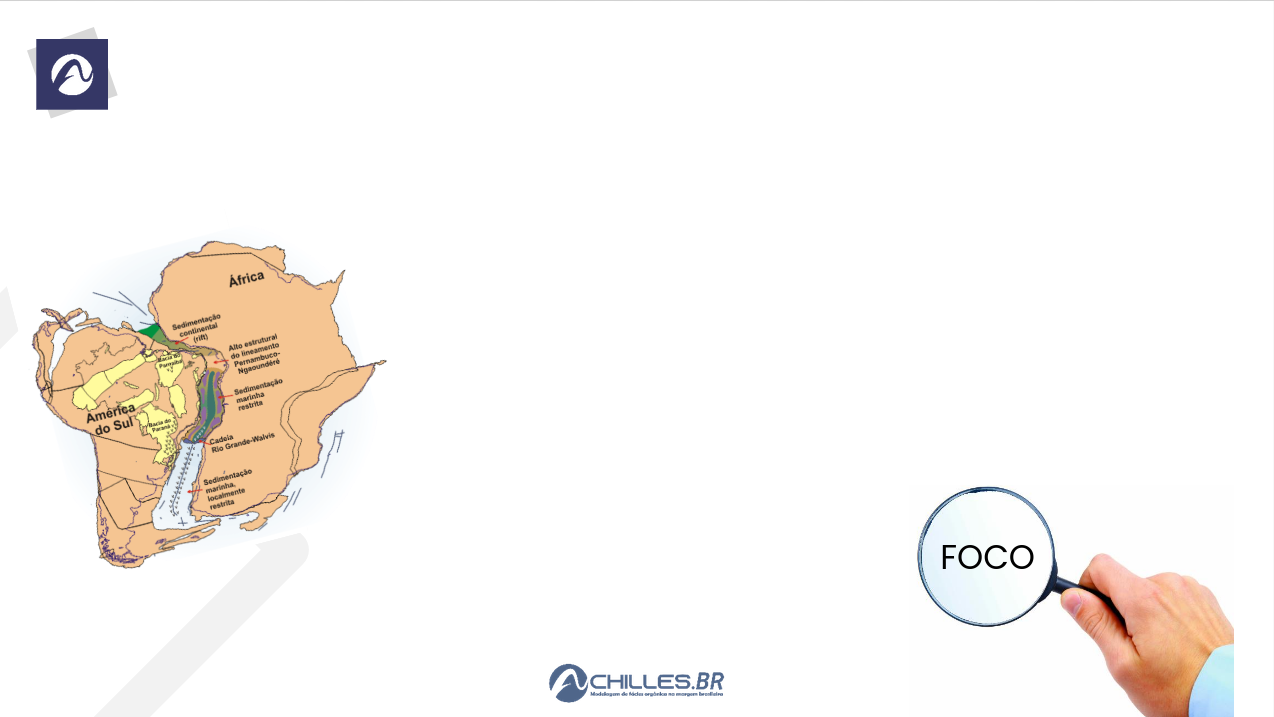
\includegraphics[width=\paperwidth,height=\paperheight]{images/sumario.png}
}

{ \begin{frame}

\begin{flushright}
Descrever o objetivo desta apresentação

\end{flushright}


\end{frame} }



%% APRESENTAÇÃO


\section{Introdução}
{
\usebackgroundtemplate{
\centering

\includegraphics[width=\paperwidth,height=\paperheight]{images/base.png}
}
\begin{frame}

\centering
Início do conteúdo da apresentação


\end{frame} 
}


{
\usebackgroundtemplate{
\centering
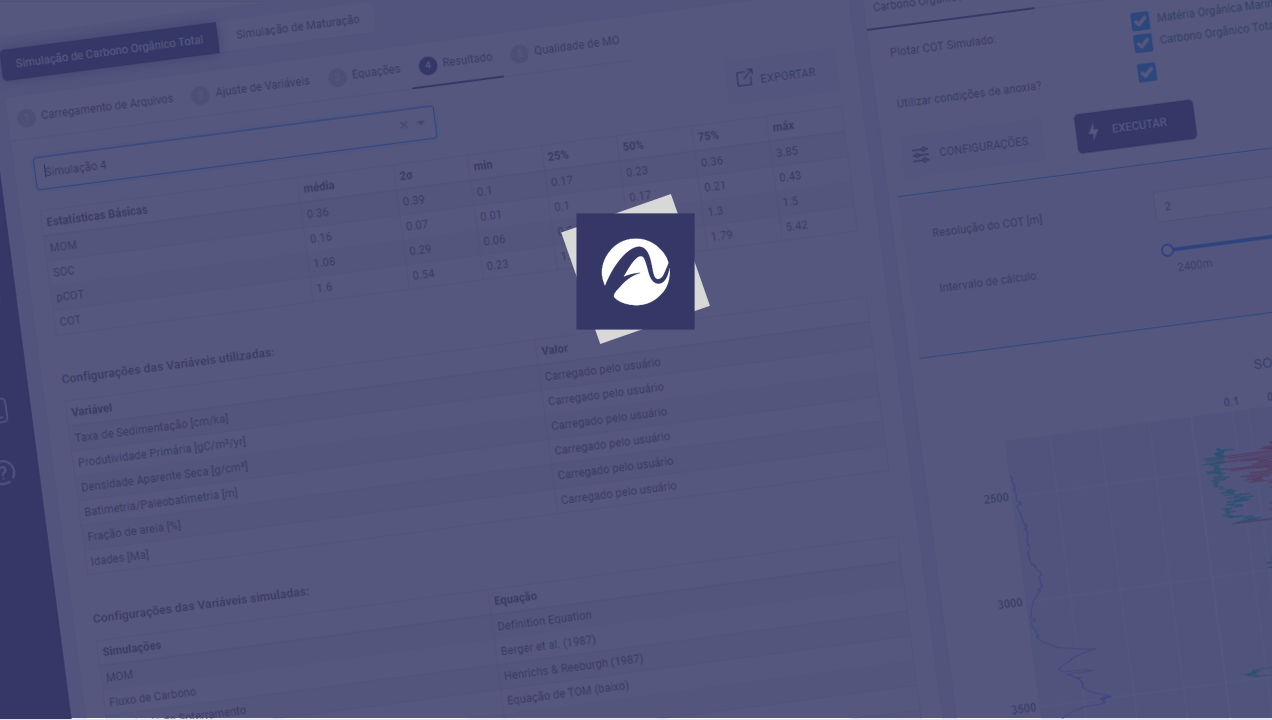
\includegraphics[width=\paperwidth,height=\paperheight]{novocapitulo.png}
}
\begin{frame}

\vspace*{3cm}
\hspace*{6.2cm}
\huge
Parte 1



\end{frame} 
}



{
\usebackgroundtemplate{
\centering

\includegraphics[width=\paperwidth,height=\paperheight]{images/base.png}
}
\begin{frame}

\centering
Início do conteúdo da apresentação


\end{frame} 
}




\section{Referencias}

{
\usebackgroundtemplate{
\centering

\includegraphics[width=\paperwidth,height=\paperheight]{images/base.png}
}
\begin{frame}[allowframebreaks]
REFERENCIAS!!!
%\beamertemplatetextbibitems
\tiny
\bibliographystyle{apalike}
\bibliography{references}
\end{frame}
}
\makeatother

{
\usebackgroundtemplate{
\centering

\includegraphics[width=\paperwidth,height=\paperheight]{images/interlocucao.png}
}
	
% Frame 3: plano de fundo
\begin{frame}

	
\end{frame}
}

{
\usebackgroundtemplate{
\centering

\includegraphics[width=\paperwidth,height=\paperheight]{images/agradecimento.png}
}
	
% Frame 3: plano de fundo
\begin{frame}
	
\end{frame}
}
\end{document}